\chapter{Energy Conversion}
\label{ch:conv}

Energy and power take many different forms, from the initial sources to the end uses. Necessarily, methods have been developed to convert energy or power from one form to another. The first method addressed in this chapter is the conversion process of thermal to mechanical to electrical energy found in heat engines and generators. This thesis is focused on geothermal heat, however, heat engines can be used with a number of different sources including the burning of a fuel such as biomass or coal, or even as waste heat from an independent process. The conversion between different forms of thermal energy and electrical power will also be discussed including electrical generators and power electronic converters that are used to form a grid in ORC prime power systems.

%This file used to contain the geothermal chapter, now contains thermal/mechanical section of the conversion chapter
\section{Thermal Energy}
Thermal energy, or heat, can originate from many different sources including combustion of a fuel, radioactive decay, or absorption of light from the sun. Heat can be used directly to warm a building, but it is also a critical step in most traditional methods of generating electrical power. 
%\chapter{Geothermal Energy}
%\label{ch:geothermal}

\subsection{Enthalpy}
Enthalpy describes the energy of a system available to be converted to work. It is related to the temperature of the geothermal resource, but also dependent on the pressure and volume. Temperature is usually the primary metric of a resource, but even a high temperature source is useless without sufficient volume flow. Quantitatively enthalpy is expressed as \cite{Nellis2009}
\begin{equation}
H = U + pV
\end{equation}
where $U$ is the internal energy, which is function of temperature, $p$ is the pressure of the system, and $V$ is the volume. Generally it is more convenient to use the change in enthalpy rather than absolute values. After a system undergoes some thermodynamic process, the system will always have some remaining internal energy, pressure, and volume. Therefore, a change in enthalpy better describes the energy extracted from (or absorbed by) the system.
Additionally, the enthalpy of a system is often normalized by the its mass for comparison to other sized systems and the mass specific enthalpy, $h$, is used instead.
\nomenclature[V]{$H$}{Enthalpy of a fluid\nomunit{\si{\joule}}}
\nomenclature[V]{$U$}{Internal energy of a fluid\nomunit{\si{\joule}}}
\nomenclature[V]{$p$}{Aboluete fluid pressure\nomunit{\si{\pascal}}}
\nomenclature[V]{$V$}{Fluid volume\nomunit{\si{\meter\cubed}}}
\nomenclature[V]{$h$}{Mass specific enthalpy of a fluid\nomunit{\si{\joule\per\kilogram}}}


\subsection{Geothermal Cycles}
%%Describe each of the following but focus on cycles for low enthalpy sources
Geothermal systems can be classified as high-, medium-, or low-enthalpy\footnote{While the technical definitions differ, the terms enthalpy, heat, and temperature are often used interchangeably when qualitatively describing geothermal sources.}. Although there is no formal delineation, high-enthalpy sources generally have temperatures greater than about $150$ \textcelsius{} ($302$ \textdegree{}F) and low-enthalpy sources have temperatures lower than $100$ \textcelsius{} ($212$ \textdegree{}F) \cite{Norden2011}. Depending on the amount of extractable energy of the resource, different geothermal processes or cycles can be used to extract the maximum amount of energy from the resource.

\subsubsection{Dry Steam}
This high-enthalpy processes extracts hot steam from the earth. The steam is sent directly through a turbine then condensed into liquid water and injected back underground. 

\subsubsection{Flash Steam} 
In the flash steam process high pressure hot water is extracted then, allowed to boil becoming steam and low pressure hot water. The steam is sent through a turbine then condensed, recombined with water, and injected back underground.

\subsubsection{Binary Cycle} 
As the name implies, binary cycles involve two loops: a heat source loop and working fluid loop. Heat is collected in the heat source loop and transferred to the working loop through a heat exchanger. The working fluid then undergoes the vaporization process to spin a turbine or other type of expander. The expander is connected to a generator which converts the rotational mechanical energy into electrical energy. After some of the heat is converted, the working fluid passes through a condenser where it is cooled further. Sometimes the cooling process involves drawing in air at ambient temperature, but it can also involve a third loop. The fluids within each of the cycles must be moved using pumps. The pumps themselves need to be powered and act as a parasitic load to the system.

Binary cycles are not limited to low or medium enthalpy heat sources. The most common binary cycle is the Rankine Cycle. A diagram of the process can be seen in \autoref{fig:rankine_cycle_diagram}. In an ideal Rankine Cycle heat is added to the working fluid under high pressure to change its phase from liquid to gas. The fluid expands isentropically\footnote{In thermodynamics, isentropic processes do not have a net change in entropy.} which rotates the generator shaft, causing the fluid's temperature and pressure to drop. Additional heat is then expelled from the fluid as it condenses at a constant low pressure side of the system. Finally the fluid is isentropically pumped back to the high pressure and the process begins again.
\begin{figure}[h]
	\centering

	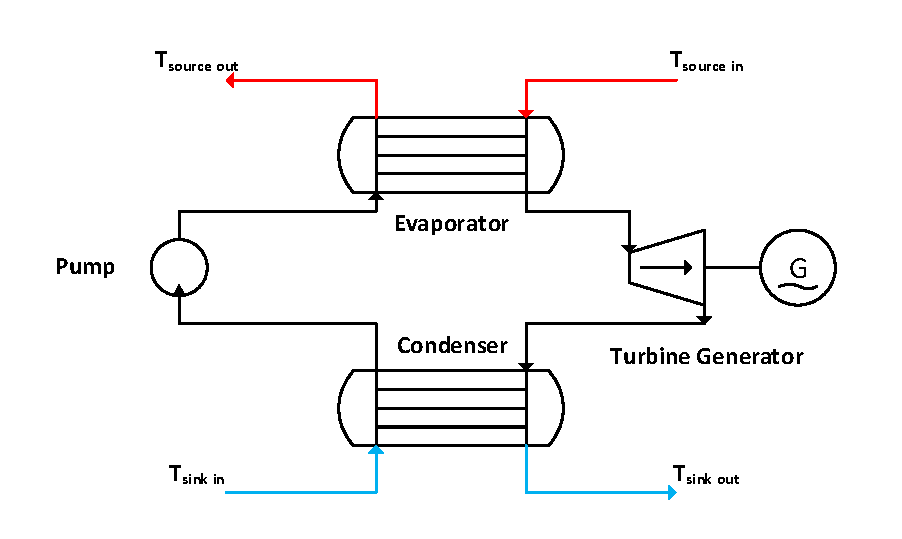
\includegraphics[width=\textwidth]{figures/RankineCycleDiagram.pdf}

	\caption{Diagram of a Rankine cycle system.}
	\label{fig:rankine_cycle_diagram}
	
\end{figure}

For geothermal sources, generally high enthalpy systems can be implemented directly with a single loop using the flash or dry steam processes. However, for lower enthalpy systems, water cannot be used as a working fluid because the temperatures are not high enough to vaporize it. In these cases an organic Rankine cycle, which uses an organic working fluid such as refrigerants instead of water, can be employed. Working fluids are typically selected for relatively low vaporization temperatures, but the thermodynamic states of the heat source must also be considered. The selection of the type of expander and pumps are discussed in Kreider \cite{Kreider}. Generally larger diameter expanders operate at lower speeds.




%\subsection{Pilgrim Hot Springs}
%Do this in 1st chapter not conv/geotherm chapter
%More thourough description of the resource and potential development plans.

 %used to contain geothermal chapter, now contains thermal section


\section{Electrical Generators}
%This section should focus the difference between the two with respect to geothermal sources. I can have a fundemental description of the generators either in this chapter or the intro chapter.
Electrical generators are spinning machines which convert the mechanical power rotating a shaft to electrical power. Fundamentally, they operate on the principles of Maxwell's and Faraday's laws which broadly state that a moving magnetic field produces an electric field and vice versa. The primary difference among generator types is how that magnetic field is produced. 
%As previously described, asynchronous generators, also called induction generators, are incapable maintaining a grid. Synchronous generators supply or absorb reactive power depending on the needs of the grid.

\subsection{Synchronous Generators}
The magnetic field in synchronous generators is formed by external sources. The name derives from the fact that electric frequency directly synchronizes with the physical rotation of the machine.\footnote{Certain wiring configurations add additional electromagnetic poles to machine which causes the mechanical speed to be slower than the electrical speed by a factor of the integer number of poles.} They are also capable of supplying reactive power because the internal magnetic field is not self induced. 

In traditional synchronous machines an electro-magnet is used to generate the field by running a DC current through the rotational, or rotor, windings. The spinning DC electric field produces a magnetic field, which in turn makes an electric field in the stationary, or stator, windings. By varying the DC current applied to the rotor, the user can control the voltage generated by the machine. The current sets the magnetic flux which in turn controls the voltage \cite{Chapman2005}. As discussed in \autoref{sec:droop}, droop control takes advantage of the relationship between voltage and reactive power to ensure they are appropriately balanced.

In permanent magnet synchronous generators (PMSG) bar magnets are used to form the magnetic field of the rotor. A benefit of using permanent magnets over electro-magnets is the lack of slip rings or brushes used to apply the DC current to the rotor winding. These components can introduce a source of friction and wear down over time. However, since permanent magnetic fields are fixed at the time of construction, the user cannot control the voltage of the machine without full power electronic conversion between the generator and the grid.
\nomenclature[B]{PMSG}{Permanent magnet synchronous generator}

\subsection{Asynchronous Generators}
Asynchronous (induction) machines generate their internal magnetic fields by self-induction rather than from an external source. Since induction machines do not rely on an additional source to operate, induction machines generally have simpler designs and are less costly than synchronous machines. However, that also means they need to consume reactive power from the grid in order to maintain their magnetic field. This field relies on the relative difference in frequency between the stator, $f_{s}$, and rotor, $f_{r}$, fields. This relative difference in frequency is represented by the machine's slip, %$s = \frac{f_{s} - f_{r}}{f_{s}}$ 
\cite{Chapman2005}
\begin{equation}
	s = \frac{f_{s} - f_{r}}{f_{s}}.
\end{equation}
\nomenclature[V]{$s$}{Slip of induction machine}

The stator frequency is equal to the grid frequency at the output terminal, while the rotor frequency is determined by the rotor's speed, $n_r$, and number of poles, where 
\begin{equation}
	f_r = \frac{n_r \times poles}{120}.
\end{equation}
The number of poles is based off the number of coil windings per phase and established at construction. When the machine's slip is positive, the field frequency in the stator is greater than in the rotor, and the machine operates as a motor. A negative slip means the rotor is spinning faster than the frequency of the stator and the machine is acting as a generator. 

Some work has been done on self-excited induction generators (SEIG) \cite{Ouazenne1983, Ammasaigounden1986}. Instead of solely consuming reactive power from the grid, induction generators use a bank of capacitors connected at their terminals to supply the necessary reactive power in order to maintain the magnetic field in the rotor. However, a significant drawback to these devices is the lack of control over frequency and voltage \cite{Bansal2005}. SEIGs require some form of power electronic conversion at the output terminals to regulate the grid side frequency and voltage. This can be achieved with full power electronic conversion, similar to PMSGs, where the generator output is entirely rectified and inverted to synchronize with the grid. Alternatively, two sets of windings can be be used around the rotor instead of one, in what is called a doubly fed induction generator (DFIG). The primary set form the stator, which connects directly with the grid\footnote{Via a transformer.} and is used to deliver power. The auxiliary set of windings are connected to the grid through a power electronic converter. This converter can be used to control the rotor current to ensure consistent frequency and voltage despite variable rotational speeds \cite{Muller2002, Bogalecka2002}.
\nomenclature[B]{SEIG}{Self excited induction generator}
\nomenclature[B]{DFIG}{Doubly fed induction generator}

\section{Power Electronic Conversion}
As described previously, electronic conversion takes electric power from either an AC or DC form and converts it to a different form or level. This is generally done by switching the path of the input current to form the desired output. Control over the switching is critical for these conversion devices. Pulse Width Modulation (PWM) and Pulse Frequency Modulation (PFM) are two alternate methods of controlling switching states of the semiconductor devices. Both methods vary the duty cycle, $D$, of the control signal of the device in order to change the on/off state. The duty cycle is the fractional time a switch is on, $t_{on}$, relative to one period of the control signal, $T$, or 
\begin{equation}
D = \frac{t_{on}}{T}. 
\end{equation}
For PWM the switching frequency is held constant while the duration of the pulse is varied to control the output. In PFM, the duration of each pulse is fixed while time between pulses, and therefore, the frequency varies.
\nomenclature[B]{PWM}{Pulse width modulation}
\nomenclature[B]{PFM}{Pulse frequency modulation}
\nomenclature[V]{$D$}{Duty cycle}
\nomenclature[V]{$t_{on}$}{Time a switch is in the on state\nomunit{\si{\second}}}
\nomenclature[V]{$T$}{Time of one period in a cycle\nomunit{\si{\second}}}
%\subsection{Linear Power Supplies}
%Linear

%\subsection{Switched Mode Power Supplies}

\subsection{DC-DC}
%description, diagram, and waveform of simple buck and boost converters
DC-DC power conversion devices can generally be divided up into three simple designs: buck to step voltage down, boost to step voltage up, and buck-boost to step voltage down or up depending on the source voltage. 
%These two designs can be combined into a single buck-boost converter capable of increasing or decreasing the voltage. 
There are additional DC-DC converter topologies which use the same concepts in these designs, but are modified to create different characteristics \cite{Mohan2003}.
%These include but are not limited to C\'uk, SEPIC, Flyback, Forward, Half-bridge, and Full-bridge converters \cite{Mohan2003}.

In a simple buck converter, seen in \autoref{fig:simple_buck}, timed switching sets the average output voltage to a value smaller than the input, or 
\begin{equation}
V_{out} = D V_{in}. 
\end{equation}
The inductor ensures a continuous current at the output and the capacitor provides an output voltage with only modest ripple. 
%Example waveforms of input and output current and voltage can be seen for a simple buck converter in fig X.

\begin{figure}[h]
	
\centering


\begin{tikzpicture}[american voltages]
\draw[color=black, thick]
%Input
(0,0) to [V, l=$V_{in}$, invert] (0,3){}

%high 
(3,3) to [L] (6,3) -- (7,3){}

%switch
(0,3) to [Tnmos] (3,3) {}

%Diode
(3,0) to [D*, *-*] (3,3){}

%low
(0,0) -- (7,0){}

%output
(7,3) to [open, l=$V_{out}$, o-o] (7,0){}
(6,3) to [C, *-*] (6,0){}
;
\end{tikzpicture}
\caption{Simplified diagram of a buck converter.}
\label{fig:simple_buck}

\end{figure}

In a simple boost converter, seen in \autoref{fig:simple_boost}, timed switching also sets the average output voltage to the desired level, but with the relationship 
\begin{equation}
V_{out} =\frac{V_{in}}{1-D}. 
\end{equation}
However, the placement of the components leads to an increasing current through the inductor while the switch is closed. When the switch is open, the relatively high current flow through the diode results in a larger average output voltage than seen at the input. As in the buck converter, the capacitor provides an output voltage with modest ripple. 
%Example waveforms of input and output current and voltage can be seen for a simple buck converter in fig X.

\begin{figure}[h]
	
\centering

\begin{tikzpicture}[american voltages]
\draw[color=black, thick]
%Input
(0,0) to [V, l=$V_{in}$, invert] (0,3){}

%high 
(0,3) to [L] (3,3) to [D*] (6,3) -- (7,3){}

%switch
(3,1.5) node[nmos] (mos) {}
(mos.gate) node[anchor=east] {}
(mos.drain) to [short, -*] (3,3){}
(mos.source) to [short, -*] (3,0){}

%low
(0,0) -- (7,0){}

%output
(7,3) to [open, l=$V_{out}$, o-o] (7,0){}
(6,3) to [C, *-*] (6,0){}
;
\end{tikzpicture}
\caption{Simplified diagram of a boost converter.}
\label{fig:simple_boost}


\end{figure}

These two topologies can be combined to form a buck-boost converter, seen in \autoref{fig:simple_buck_boost} which has an input/output voltage relationship of 
\begin{equation}
V_{out} = V_{in}\frac{D}{1-D}. 
\end{equation}
This configuration allows the output voltage to be either greater than the input voltage for $D > 0.5$ or less than the input voltage for $D < 0.5$. It must be noted that while this orientation gives a greater voltage range at the output, the output voltage has a negative polarity. With appropriate electrical isolation, the polarity should not impact the operation of the buck-boost converter, but using a common ground between the input and output will cause the circuit to fail.

\begin{figure}[h]
	
\centering


\begin{tikzpicture}[american voltages]
\draw[color=black, thick]
%Input
(0,0) to [V, l=$V_{in}$, invert] (0,3){}

%high diode
(7,3) -- (6,3) to [D*, *-*] (3,3){}

%switch
(0,3) to [Tnmos] (3,3) {}

%inductor
(3,0) to [L, *-*] (3,3){}

%low
(0,0) -- (7,0){}

%output
(7,0) to [open, v=$V_{out}$, o-o] (7,3){}
(6,3) to [C, *-*] (6,0){}
;
\end{tikzpicture}
\caption{Simplified diagram of a buck-boost converter.}
\label{fig:simple_buck_boost}

\end{figure}

\subsection{Rectifier and Inverter}
%description, diagram, and waveform of simple rectifier
Simple rectifiers use a combination of diodes to convert an AC voltage to DC. \autoref{fig:3ph_rectifier} shows a simple example of a three phase rectifier. The diodes allow a path such that the DC current always flows in the same direction regardless of AC polarity. More advanced designs will use active switching devices and a control scheme to provide the same function. Though more complicated to implement, the user has more direct control over the output as well as how the load appears to the input. 
%Example waveforms of input and output current and voltage can be seen for a simple buck converter in fig X.
\begin{figure}[h]
	
\centering

\begin{tikzpicture}
\draw[color=black, thick]
% AC leads
% Wye neutral
(0,2) -- (0,5)

% Three phase voltage sources
(0,5) to [sV, l=$v_A$] (2,5) to [short, -*] (3,5){}
(0,3.5) to [sV, l=$v_B$, *-] (2,3.5) to [short, -*] (4.5,3.5){}
(0,2) to [sV, l=$v_C$] (2,2) to [short, -*] (6,2){}

% A ph diodes
(3,0) to [D*] (3,2) -- (3,5) to [D*] (3,7){}

% B ph diodes
(4.5,0) to [D*, *-] (4.5,2) -- (4.5,5) to [D*, -*] (4.5,7){}

% C ph diodes
(6,0) to [D*, *-] (6,2) -- (6,5) to [D*, -*] (6,7){}


%DC leads
(3,7) to [short, -o] (9,7){}
(3,0) to [short, -o] (9,0){}

%Output 
(8,7) to [C, *-*] (8,0){}
(9,7) to [open, l=$v_{dc}$] (9,0)
;
\end{tikzpicture}

\caption{Simplified diagram of a three phase full-bridge rectifier.}
\label{fig:3ph_rectifier}

\end{figure}


%\subsection{Inverter}
%description, diagram, and waveform of simple inverter
Inverters function as rectifiers in reverse. A DC source is switched on and off such that it alternates periodically. The three phase inverter diagram, seen in \autoref{fig:3ph_inverter}, is similar to the rectifier diagram, except the inverter must use active switching. In fact many inverters are designed to be reversible. The device can control the flow of active and reactive power in inverter mode or rectifier mode.
\begin{figure}[h]
	
\centering

\begin{tikzpicture}
\draw[color=black, thick]
%DC leads
(0,0) -- (7,0){}
(0,7) -- (7,7){}

%Input 
%(1,7) to [C, *-*] (1,0){}
(0,7) to [V, l_=$v_{dc}$] (0,0)

%A switches
(3,5.5) node[nmos] (mos) {}
(mos.gate) node[anchor=east] {}
(mos.drain) to [short, -*] (3,7){}
(mos.source) -- (3,4.5) to [short, *-o] (10,4.5) to [short, l_=$v_{A}$] (10,4.5){}

(3,1.5) node[nmos] (mos) {}
(mos.gate) node[anchor=east] {}
(mos.drain) -- (3,4.5){}
(mos.source) to [short, -*] (3,0){}

%B switches
(5,5.5) node[nmos] (mos) {}
(mos.gate) node[anchor=east] {}
(mos.drain) to [short, -*] (5,7){}
(mos.source) -- (5,3.5) to [short, *-o] (10,3.5) to [short, l_=$v_{B}$] (10,3.5){}

(5,1.5) node[nmos] (mos) {}
(mos.gate) node[anchor=east] {}
(mos.drain) -- (5,3.5){}
(mos.source) to [short, -*] (5,0){}

%C switches
(7,5.5) node[nmos] (mos) {}
(mos.gate) node[anchor=east] {}
(mos.drain) -- (7,7){}
(mos.source) -- (7,2.5) to [short, *-o] (10,2.5) to [short, l_=$v_{C}$] (10,2.5){}

(7,1.5) node[nmos] (mos) {}
(mos.gate) node[anchor=east] {}
(mos.drain) -- (7,2.5){}
(mos.source) -- (7,0){}


;
\end{tikzpicture}

\caption{Simplified diagram of a three phase inverter.}
\label{fig:3ph_inverter}

\end{figure}

Depending on how the inverter is expected to interact with other components on the grid, different control schemes may be needed to shape the output signal appropriately. When operating in a grid-forming mode, the inverter must be capable of regulating the frequency and voltage and is called a voltage source inverter (VSI) \cite{Engler}. When an inverter is operating in grid-following mode, it uses the grid to set its output frequency and voltage and supplies power based on active and reactive power setpoints. Grid-following inverters are also called current source inverters (CSI). Grid-supporting units usually assist the grid-forming source or inverter with frequency and voltage regulation often using droop or similar methods of control as discussed in \autoref{sec:droop}. Lastly, grid-parallel inverters supply power based off of references at the input instead of the grid, and are often used with wind turbines and solar PV arrays to provide the maximum power possible \cite{Mohd2009}.
\nomenclature[B]{VSI}{Voltage source inverter}
\nomenclature[B]{CSI}{Current source inverter}

\subsection{AC-DC-AC}
In certain situations, full power electronic conversion is necessary, where an AC source is rectified to DC, then inverted back to AC at the output. This is done when the power source is generating unregulated AC, such as with SEIGs and PMSGs, but the grid or load requires regulated AC \cite{ALOLAH1994111, Seung-HoSong2003}. In other instances, either end of the converter is regulated independently, so a DC link is required to exchange power, such as with DC interties \cite{Okada}.

\section{ORC Manufacturers and Developers}
A partial list of ORC system developers can be seen in \autoref{tab:orc_manufacturers_dev} with fewer than ten documented installed systems. A list of commercial systems with more than ten documented systems installed can be seen in \autoref{tab:orc_manufacturers_com}. Both tables also include, if available, the working fluid used, the mechanical drive, the approximate maximum rotational speed, the generator type, and the rated output. These tables show R245-fa\footnote{\ch{CF3CH2CHF2} (1,1,1,3,3- pentafluoropropane)} is commonly used as a working fluid among these manufacturers. Furthermore, these devices mostly use induction machines or PMSGs, although there is a documented instance using a DC generator. For the machines using PMSGs, a grid-following electronic conversion device is used to convert the generator output to match that of the grid, while the induction generators connect directly to the grid for a source of reactive power and to regulate their frequency and voltage.
\begin{table}
\centering
\caption{Manufacturers and developers of ORCs under development with less than ten documented installed systems. Also listed are the working fluids, mechanical drives, approximate rated operating speed, generator type, and rated output.}
\label{tab:orc_manufacturers_dev}
\rowcolors{1}{white}{gray!25}

\begin{tabular}[c]{p{2.7cm}p{2.8cm}p{2.0cm}p{1.5cm}p{1.6cm}p{2.0cm}}%{lllrlr}%
	\toprule
	%\multicolumn{6}{c}{ \multirow{2}{*}{\textbf{Under Development} (fewer than 10 documented installed systems)}}	\\ \midrule
	%\multicolumn{6}{c}{ \textbf{Under Development} (fewer than 10 documented installed systems)}	\\ \midrule
	%\multicolumn{6}{c}{}	\\ \hline
	%\rowcolor[gray]{5}
	\textbf{Company}		& \textbf{Working Fluid}		& \textbf{Mech. Drive} 		& \textbf{Rated RPM}	& \textbf{Gen. Type}	& \textbf{Size (kW)}  \\
	\midrule
	Air Squared				& 									& Scroll					& 2600 			& 						& 12 \\ 
	Termo2Power				& R245-fa							& Rotary Lobe				& 				& 						& \numrange{10}{300} \\ 
	Climeon					& 									& Turbine					& 				& 						& 150 \\ 
	Calnetix/ Access Energy	& R245-fa							& Turbine					& 30000			& PMSG					& 120 \\ 
	Verdicorp				&									& Turbine					& 45000			& PMSG 					& \numrange{65}{380} \\ 
	Inifinity Turbine		& R245-fa, supercrit. \ch{CO2}		& Radial Outflow Turbine	& 3600			& Induction \& DC 		& \numlist{10;50} \\ 
	Ener-G-Rotors			& 									& Trochoidal Gear Engine using ge-rotor &	&  						& \numlist{40;60} \\ 
	Phoenix					& R245-fa, Novec-649, Cyclohexane	& 							& 				& 						& \numlist{25;50;100;250} \\ \bottomrule
\end{tabular}
\end{table}
	
\begin{table}
\centering
\caption{Manufacturers and developers of commercial ORCs with more than ten documented installed systems. Also listed are the working fluids, mechanical drives, approximate rated operating speed, generator type, and rated output.}
\label{tab:orc_manufacturers_com}
\rowcolors{1}{white}{gray!25}	
\begin{tabular}[c]{p{3.0cm}p{2.5cm}p{2.0cm}p{1.5cm}p{1.6cm}p{2.0cm}}%{lllrlr}%
	\toprule
	\textbf{Company}          & \textbf{Working Fluid}		& \textbf{Mech. Drive}			& \textbf{Rated RPM}	& \textbf{Gen. Type}	& \textbf{Size (kW)}  \\
	\midrule
	Electratherm              & R245-fa 					& Twin Screw 					& 5000				& Induction  			& \numlist{35;65;110} \\ 
	E-Rationale               & R245-fa, SES36 				& Single Screw Radial Inflow	& 3600				& Induction				& \numlist{55;75;110;132} \\ 
	Exergy                    &								& Radial Outflow Turbine		&            		& 						& 125 and up \\ 
	Zuccato                   & Hydrofluoro-carbon mixture	& Radial Inflow Turbine			& 18000				& PMSG 					& \numlist{30;40;50} \\ 
	Enogia                    & R245-fa						& Turbine 						& 					& 						& \numlist{10;20;40;100}\\ 
	Clean Energy Technologies & R245-fa						& Turbine 						& 27500				& 						& 125 \\ 
	Tri-O-Gen                 & 							& Turbine 						& 					& 						& 165 \\ \bottomrule

\end{tabular}
\end{table}

\begin{comment}
%\subsection{ORC Manufacturers and Developers}
%\subsubsection{Under Development}
\begin{description}
	\item[Air Squared] Expander: Scroll expander based on automotive scroll compressor.
	\item[Termo2Power] Working fluid: R245fa. Expander: Rotary Lobe expander
	\item[Climeon] Expander: turbine expander.
	\item[Calnetix/Access Energy] Working fluid: R245fa. Expander: turbine expander
	\item[Verdicorp] has a range of variable speed expanders. The expander connects to the rotor of a permanent magnet synchronous generator. An IGBT variable frequency drive converts and synchronizes the power with a local grid. Expander: Turbine expander based on Dunfoss Turbocor compressor
	\item[Inifinity Turbine] 50kW Working fluid: R245fa -- 10kW Working fluid: supercritical $CO_2$. Expander: Radial Outflow Turbine
	\item[Ener-G-Rotors] Expander: Trochoidal Gear Engine using ge-rotor
	\item[Phoenix] Working fluid: R245fa
\end{description}
%\subsubsection{Commercial Products}
\begin{description}
	\item[Electratherm] makes use of a twin screw expander to spin an induction generator.  Working fluid: R245fa. Expander: Twin screw expander
	\item[E-Rationale] uses a single screw expander to rotate an induction generator. Working fluid: R245fa or SES36. Expander: Single screw expander
	\item[Exergy] Expander: Radial outflow turbine
	\item[Zuccato] uses a radial inflow turbine directly connected to synchronous permanent magnet generator. Electric power is converted and synchronized to local power grid with IGBT switching. Expander: Radial inflow turbine
	\item[Enogia] uses a turboexpander. Electric power is rectified then tied into the grid with a grid feed inverter. Working fluid: R245fa. Expander: Turbine expander
	\item[Clean Energy Technologies] %uses high speed turbine. Working fluid: R245fa. Expander: Turbine expander
	\item[Tri-O-Gen] %uses high speed turbine 
\end{description}
\end{comment} 
\nomenclature[B]{R245-fa}{Working fluid \ch{CF3CH2CHF2} (1,1,1,3,3- pentafluoropropane)}

\cleardoublepage